\documentclass[11pt]{article}

\usepackage{fullpage}
\usepackage[utf8]{inputenc}

\usepackage{algorithm}
\usepackage{algorithmic}

\usepackage{amsmath}
\usepackage{amsfonts}
\usepackage{amssymb}
\usepackage{graphicx}
\usepackage{float}
\usepackage{amsthm}
\usepackage{enumitem}

\newtheorem{Lemma}{Lemma}
\newtheorem{Theorem}{Theorem}


\title{Optimally Gathering Two Robots}
\author{Some smart people}
\date{April 2017}

\graphicspath{{../png/}}


\begin{document}

\maketitle

\section{Introduction}

\subsection{Problem Definition}


The gathering problem for two robots is achieved in a self-stabilizing fashion in finite time if and only if, for any starting position, phase and colour, after a finite number of activations, both robots are located at the same coordinates.



\subsection{Model}

We consider a system of two robots modelled as mobile points in the plane $\mathbb{R}^2$.

Both robots execute cycles of three phases : LOOK, COMPUTE AND MOVE. When a robot is not executing a LOOK-COMPUTE-MOVE (LCM) cycle, it is considered to be in a WAIT phase.

\begin{itemize}
\item WAIT : The robot is idle and waiting for activation.
\item LOOK : The robot is taking a snapshot of the positions of the other robots. This phase is assumed instantaneous.
\item COMPUTE : The robot computes its next destination using the snapshot. 
\item MOVE : The robot moves towards its destination.

\end{itemize}

We assume the COMPUTE and MOVE phases have an unknown, but finite duration, which is decided by the scheduler.
\\
Robots are anonymous, meaning they are indistinguishable and they execute the exact same algorithm. However, for the sake of practicality, they are called A and B. Note that switching their name during the proof has no consequence on its correctness.
\\
Each robot runs a different coordinate system about which we make no assumptions. We also assume that robots have no mean of explicitly communicating with each other.
\\
The robots are also oblivious, which implies the COMPUTE phase can have no other input than the snapshot from the LOOK phase.
\\
We consider a fair, asynchronous scheduler. This means that both robots must be activated infinitely often. This also implies that the scheduler can activate a single phase of a robot.
At every instant, the scheduler can activate either A, B or both.



Regarding the MOVE phase, we call $\delta$ the minimum distance a robot can travel through a single MOVE phase if its target is farther than delta. If the target of the robot is closer than $\delta$ when the robot activates its MOVE phase, then we assume the robot reaches its target.

In other words, if a robot has a target at a distance $x$, we assume that, at the end of its move phase, the robot has moved a distance in $[min(\delta,x),x]$. The exact position reached is determined by the adversary scheduler.

The current discussed model has already be proven to be insufficient to achieve two-robot gathering by [Suzuki Yamashita].

Following the work of [Das Flocchini Prencipe Santoro Yamashita] we consider a similar model of robot, this time fitted with a light.
\\
Each robot is able to include the other's color in its snapshot. Each robot is also now able to consider its own color as a second input of its COMPUTE phase. In other words, robots are now able of storing and using a finite number of bits of shared memory.
\\
A robot is able to change the colour of its own light at the end of its COMPUTE phase, i.e. at the moment of the activation of its following MOVE phase.
\\
as proven in [Das Flocchini Prencipe Santoro Yamashita], having four colours (i.e. two bits of shared memory) allows for an asynchronous two robot gathering.
\\
We now consider the robots to be fitted with only two colours (i.e. one bit) called black and white.

In [Viglietta], it has been proven that three colours and the ability to detect null distances is also sufficient for an asynchronous, non rigid scheduler.

\subsection{Our contribution}

In this paper, we show and prove an algorithm that is able to solve the gathering problem for two robots in a self-stabilizing fashion in finite time using only two colours.

As proven in [Viglietta], no two colour algorithm can solve the gathering if the computation relies on this form of calculation :

$$ me.destination = (1-\lambda ) \cdot me.position + \lambda \cdot other.position $$

With :

$$ \lambda = f(me.colour, other.colour)$$

As such, we do not assume all computation to be of this form and show that superposition detection is sufficient to ensure two robot gathering.

\section{Proposed Algorithm :}
\subsection{Problem}

As explained with more details in [Viglietta], to solve the problem, a gathering algorithm needs to make sure of three things : 

\begin{itemize}
\item If the robots are synchronized, they need to move towards the middle point
\item If the robots are not synchronized, one needs to move towards the other
\item In that case, the other robot must not move (only necessary in ASYNC)
\end{itemize}

\subsection{Algorithm}
We consider the following algorithm :

\begin{figure}[H]
	\centering
	\includegraphics[width=0.8\linewidth]{Algorithm.png}
	\caption{Existing Algorithm}
\end{figure}

This is the algorithm used to solve non-rigid SSYNC in [Viglietta] and which cannot solve non-rigid ASYNC.

We introduce a slight change in behaviour in the white state :

\begin{figure}[H]
	\centering
	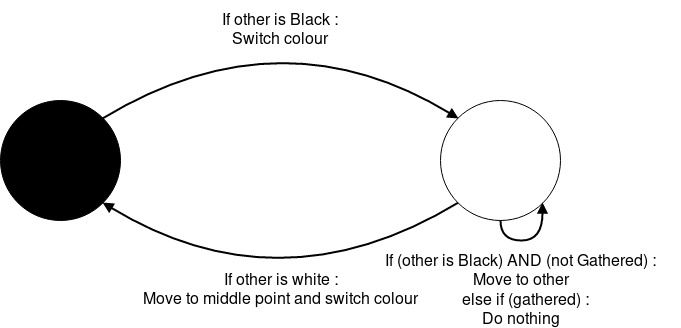
\includegraphics[width=0.8\linewidth]{Algorithm2.png}
	\caption{Proposed Algorithm}
\end{figure}

\begin{algorithm}
\caption{Robot Algorithm}         
\label{alg1}                           
\begin{algorithmic}                    
    \STATE 
    \IF{me.colour = white \AND other.colour = white}
        \STATE me.destination $\Leftarrow$ other.position/2 + me.position/2
        \STATE me.colour $\Leftarrow$ black
    \ELSIF{me.colour = black \AND other.colour = black}
        \STATE me.colour $\Leftarrow$ white
    \ELSIF{me.colour = white \AND other.colour = black \AND (me.position $\neq$ other.position)}
        \STATE me.destination $\Leftarrow$ other.position
    \ENDIF
\end{algorithmic}
\end{algorithm}


\begin{Theorem}
The proposed algorithm solves the gathering problem for two robots in a self-stabilizing fashion in finite time for the non-rigid ASYNC model.
\end{Theorem}

\subsection{Principle}

The principle of the algorithm is the following :

If both robots A and B start in the same colour and are fully synchronized, they move along the white to black and black to white vertexes. In that case, the each move towards the middle point.

If they get de-synchronized or start in different colours, the robot in black is forced to stay put while the robot in white moves towards it on the white to white vertex.

If a robot executes a compute phase with a snapshot showing both robots at the same location, it will not execute a MOVE phase (or an infinitely short MOVE phase with no destination).

We will directly prove the algorithm for the ASYNC model. 
This requires us to take into account what exactly happens during the de-synchronisation.


\section{Proving the algorithm :}

\subsection{Introduction}

To prove this algorithm for the ASYNC model, we need to consider every possible configuration of the algorithm.
\\
We consider the different types of phases that can be reached by the algorithm : 
\begin{figure}[H]
	\centering
	\includegraphics[width=0.8\linewidth]{Cases.png}
	\caption{Configurations}
\end{figure}

\begin{itemize}
\item W : Wait
\item C2H : Compute to Half (at the end of this compute phase, the robot switches its colour to black and moves towards the middle point)
\item C2O : Compute to Other (at the end of this compute phase, the robot stays white and moves towards the other robot)
\item M2O : Move to Other robot's position
\item C2W : Compute to White (compute phase that leads to colour change and no motion)
\item C2B : Compute to Black (compute phase that leads to no colour change and no motion)
\item M2H : Move to Half point
\item C2N : Compute to Nothing (compute phase that leads to no motion)
\end{itemize}

Since robots are anonymous, we only need to consider half of the possible configurations (i.e. [W,C2H] == [C2H,W]). 

The named configurations (i.e. A1, F4 ...) will be used as targets in the configuration graphs. 

The configurations with yellow backgrounds pose an interesting problem :
In those cases, the simultaneous activation of A and B by the scheduler is not perfectly defined. Indeed, activating A then B or B then A does not lead to the same configuration. In those cases, we need to consider two different simultaneous activations.
\\

We then divide the complete set of configurations in six subsets :

\begin{enumerate}[label=(\alph*)]
\item SYM : configurations where A and B are in, or can reach, identical states.
\item ASYM : configurations where A and B are differentiated into a black robot and a white robot and have no way of going back to being identical.

These two subsets cover the normal operation of the algorithm.

\item FAULTY 1 : faulty configurations after a white to black de-synchronisation.
\item FAULTY 2 : faulty configurations after a black to white de-synchronisation.

These two subsets cover faulty behaviour allowed by the algorithm.

\item ILLEGAL : configurations that cannot be reached by the algorithm but need to be taken into account as possible starting configurations to prove self-stabilization
\item GATHERED : Specific configurations that can only be reached if the gathering is complete.
  

\end{enumerate}


Each subset is drawn as a graph of its configurations and the possible exits. Some entrances of FAULTY 1 and FAULTY 2 are also represented for better readability.

Each graph is divided in two parts : the top part, called nominal behaviour and a bottom part called terminal behaviour. 

The behaviour of the algorithm is called nominal when a robots are not gathered. Certain nodes, represented in the bottom part, will change their behaviour if the gathering is achieved during their activation. This is the case when a white robot activates its look phase and perceives the other robot and itself on the same coordinates. Specific gathered behaviour is called terminal.



\pagebreak
\begin{figure}[htb]
	\centering
	\includegraphics[scale=0.44]{SYM.png}
	\caption{SYM configurations}
\end{figure}
\pagebreak

\begin{figure}[htb]
	\centering
	\includegraphics[scale=0.7]{ASYM.png}
	\caption{ASYM configurations}
\end{figure}
\pagebreak

\begin{figure}[htb]
	\centering
	\includegraphics[scale=0.6]{Faulty_1.png}
	\caption{FAULTY 1 configurations}
\end{figure}
\pagebreak

\begin{figure}[htb]
	\centering
	\includegraphics[scale=0.6]{Faulty_2.png}
	\caption{FAULTY 2 configurations}
\end{figure}
\pagebreak

\begin{figure}[htb]
	\centering
	\includegraphics[scale=0.6]{Illegal.png}
	\caption{Illegal configurations}
\end{figure}
\pagebreak

\begin{figure}[htb]
	\centering
	\includegraphics[scale=0.5]{Gathered.png}
	\caption{Gathered configurations}
\end{figure}
\pagebreak

\begin{figure}[htb]
	\centering
	\includegraphics[scale=0.7]{Legend.png}
	\caption{Graph legend}
\end{figure}
\pagebreak

\begin{figure}[htb]
	\centering
	\includegraphics[scale=0.6]{Legend_2.png}
	\caption{Graph Legend}
\end{figure}
\pagebreak

\subsection{Proof}


To prove the correctness of the algorithm, we need to prove that : 

\begin{itemize}
\item every nominal behaviour leads to a terminal phase (i.e. a gathered configuration)
\item every terminal phase leads to the robots eventually staying in a gathered configuration infinitely.
\end{itemize}

for every subset of configurations. A subset is called valid once these two properties have been proven.
\begin{Lemma}
If every subset of configurations is valid, then the algorithm is valid.
\end{Lemma}


\textit{Proof :} \textbf{Je sais pas si c'est vraiment nécessaire de prouver ça ? }


\begin{Lemma}
Every subset of configurations is valid.
\end{Lemma}

\textit{Proof :} To prove this, we proceed in order : We first prove the validity of ASYM, which is the easiest. We then prove that FAULTY 1 can only lead to ASYM and is therefore valid. After that, we prove the validity of SYM with similar reasoning, excluding the exit to FAULTY 2. The hardest part is now to prove FAULTY 2, assuming SYM is valid, which we previously proved. It is then quite trivial to prove ILLEGAL and GATHERED

\subsubsection{ASYM}

\begin{Lemma}
The ASYM subset is valid.
\end{Lemma}


\textit{Proof :} ASYM is the subset that is reached after a successful de-synchronization of A and B where A and B are now differentiated into a white and a black robot.

It is the easiest subset to prove. Indeed, as it has no possible exits. We can easily prove that, once the system is in a ASYM configuration, in nominal behaviour, fair activations of the robots will lead to :

\begin{itemize}
\item A moving towards B
\item B not moving
\end{itemize}


It is therefore easily proven that the nominal behaviour leads to both robots sharing the same coordinates in a finite number of steps.
Once it is done, the following activation of robot A leads to either the B1 or B2 configuration. The following activation of A then leads to either F5 or F7, which, in turn, either leads to B1 or B2. The system, is now stuck in a no-movement loop.

Therefore, the ASYM subset of configuration is a valid subset.

\subsubsection{FAULTY 1}

\begin{Lemma}
The FAULTY 1 subset is valid.
\end{Lemma}


\textit{Proof :} the FAULTY 1 subset is reached with a white to black de-synchronization.
It is then possible to have robot A moving towards the middle point and B moving towards A.

The first thing to notice in the FAULTY 1 subset is that, in nominal behaviour, the system can only exit the subset by going to the ASYM subset, which we have proven to be a valid subset.
It is also worth noticing that, while three cycles exist in this subset, none of them can actually be kept under the fair scheduler assumption, i.e. it would require one robot to never be activated. And, while it is possible to switch from the first cycle to the second, and from the second to the third, breakage of the third cycle leads the system to the ASYM subset.

Therefore, the nominal behaviour of FAULTY 1 is valid.

Note that the only configuration of FAULTY 1 whose behaviour is modified by achieving the gathering is C1. C1 can then lead to either B1 and ASYM, or F5 and ASYM. Finally, if only the white robot is activated, it is possible to cycle between C1 and F8. However, the fair scheduler assumption requires this cycle to be broken and the system to move to the ASYM subset.

We can conclude that, despite being an faulty subset, FAULTY 1 is merely a temporary subset, provided the scheduler is fair.

\subsubsection{SYM}

\begin{Lemma}
If we exclude the path to FAULTY 2, the SYM subset is valid.
\end{Lemma}

\textit{Proof :}  the SYM subset is considered the normal starting starting subset (A and B waiting in white). It comprises the FSYNC states (A1 to A1 through simultaneous activations) and every state that can be reached by A1 and lead back to A1 (except through FAULTY 2).  

In this subset, it is possible to exit through ASYM, FAULTY 1 or FAULTY 2. It is also possible to cycle through SYM. This can either be done from A6 to A2, A7 to A5 or by cycling back to A1. In each case, cycling through SYM implies both robots targeting the middle point while not moving, and then both of them moving towards the middle point. This behaviour is then valid.

We have already proven ASYM and FAULTY 1 to be valid. Therefore, SYM nominal behaviour is valid if we do not consider FAULTY 2.

Achieving the gathering implies terminal behaviour for nodes A1, A2, A3, A4 and A6.
\\

Possible terminal behaviour is :

\begin{itemize}
\item A1 can lead to F1 which leads to A1 
\item A1 can lead to F9 which leads to A1 

\item A2 can lead to ASYM
\item A2 can lead to F2 or F8 which leads to A2, FAULTY 1 or ASYM

\item A3 can lead to F3 or F4 which leads to A3, A4 or A1
\item A3 can lead to A4 

\item A4 can lead to A1
\item A4 can lead to F1 which leads to A1 
\item A4 can lead to F4 which leads to A1 or A4

\item A6 can lead to A1 
\item A6 can lead to F1 which leads to A1 
\item A6 can lead to F6 which leads to A1 or A6
\end{itemize}

For one, it is clear that it is no longer possible to reach FAULTY 2, as neither A6 nor A2 can lead to their faulty targets any longer. Furthermore, Reaching A2 with an invalid target after achieving the gathering now will lead to FAULTY 1 or ASYM, which are valid subsets. Looping around to A2 would, indeed, require an unfair scheduler.
\\
It is also clear that, once the gathering is complete, SYM can either loop without motion or lead to a valid subset. Therefore, SYM has a valid terminal behaviour.
\\
Therefore, SYM, excluding FAULTY 2, is a valid subset.

\subsubsection{FAULTY 2}

\begin{Lemma}
The FAULTY 2 subset is valid.
\end{Lemma}

The FAULTY 2 subset is reached with a black to white de-synchronization.
It is then possible to have robot A moving towards B and B targeting the middle point.

This is the subset that actually defeats the algorithm in [Viglietta]. We need to prove that our algorithm cannot be defeated in the same way.

FAULTY 2 poses quite a problem : It is possible to enter FAULTY 2 from A6 in the SYM subset. However, it is also possible to exit FAULTY 2 to A2 in SYM. This A2 configuration contains an abnormal target. Therefore, it is possible for a scheduler to create a FAULTY 2 $<->$ SYM cycle.

We need to prove that this particular cycle does not threaten the gathering. 

\begin{Lemma}
The FAULTY 2 $<->$ SYM cycle reduces the distance between A and B.
\end{Lemma}


\textit{Proof :} we notice that, in order to keep this cycle running, we need to go through the A6 configuration, and then the A2 configuration.

If we assume that, in the A6 configuration, we have :
\begin{itemize}
\item A, white, in position 0 with no target
\item B, black, in position x with no target

\end{itemize}

Then it is possible to prove, by exploring every possible path, that when reaching A2  :

\begin{itemize}
\item A is in position $[min(\delta,x),x]$ with no target
\item B is in position x with either $\dfrac{x}{2}$ or $[\dfrac{x}{2},x]$ as a target.
\end{itemize}

Now, to go back to A6, the system first needs to exit A2, which necessarily makes A target the middle point between A and B. It then needs to execute both targets. 
This means that, when back to A6, the distance between A and B is now $[-\dfrac{x}{2},x-3\delta]$ which is less than x.
\\
Because of this, a scheduler using a FAULTY 2 $<->$ SYM cycle cannot prevent A and B from moving closer to each other. 
\\
If the distance x in the A6 configuration is inferior to $\delta$, then at the end of D2, the gathering is achieved, as A would have moved to B.

Therefore, the nominal behaviour of FAULTY 2 is valid.

FAULTY 2 does not have a terminal behaviour. We can, however, note that in terminal behaviour, A2 cannot lead to A6 (proved in the SYM section). This means that the FAULTY cycle leads to the gathering, and is then broken when reaching A2.
\\
Therefore, FAULTY 2 is a valid subset.
\\
Because of this, SYM is also a valid subset.

\subsubsection{Illegal}
\begin{Lemma}
The ILLEGAL subset is valid.
\end{Lemma}


\textit{Proof :}
This subset covers configurations that are not possible to reach from normal behaviour. This is necessary to ensure self-stabilization. 
We can quickly notice that no cycle exists within the illegal subset and that this subset needs to exit to either SYM or FAULTY 1.

Therefore, this subset is valid.

\subsubsection{Gathered}

This subset has actually already been proven above in the different subset of which it is the terminal behaviour.

\subsubsection{Self-Stabilization}

To prove the algorithm works in a self-stabilizing fashion, we need to prove that every possible starting configuration leads to a valid gathering. To do so, we need to prove two things : 

\begin{itemize}
\item Starting from anywhere leads to gathering
\item No false target can be kept indefinitely
\end{itemize}

This second hypotheses is necessary as we do not take the target into account in the configurations.

We already proved that every subset of configurations is valid and leads to the gathering. 
\\
To prove that no target can be kept infinitely in the general execution, we only need to prove it for SYM and ASYM, as all other subsets eventually lead to either of them.
\\
This proof is quite trivial for ASYM, as it is a cycle of motion for the white robot.
\\
For SYM, we notice that cycling through the subset requires moving from the leftmost configurations (A1-2-9) to the rightmost configurations. this implies crossing the yellow-bubbled configurations and, again, provided the scheduler is fair, activating both robots through their MOVE phase once. This implies that no target acquired before can be kept is the right part of the graph.
\\

As we have proven, every subset is valid. We also proved self-stabilization. It is then proven that this particular algorithm solves the gathering problem for two robots in a self-stabilizing fashion in finite time for the non-rigid ASYNC model.

\section{Conclusions}

In this paper we introduced a new algorithm which solves the gathering problem for two robots in a self-stabilizing fashion in finite time for the non-rigid ASYNC model. This algorithms uses both colour and distance information from the snapshot. Proving this algorithm required extensive exploring of the possible configurations of the execution.


\end{document}
